% Source: AESP_466_ClassWork/Supplements/Companion/Euler_Sequences_Quaternions/Euler_Sequences_Quaternions.tex

\documentclass[border=4pt]{standalone}
\usepackage{amsmath}
\usepackage{amssymb}
\usepackage{graphicx}
\usepackage{tikz}
\usepackage{xcolor}
\usetikzlibrary{shapes.geometric, arrows.meta, positioning, decorations.pathmorphing, decorations.pathreplacing, patterns, calc, 3d}

\definecolor{Garnet}{HTML}{73000A}
\definecolor{USC_Rose}{HTML}{CC2E40}
\definecolor{USC_Blue}{HTML}{466A9F}
\definecolor{USC_Slate}{HTML}{1F414D}
\definecolor{USC_Olive}{HTML}{65780B}
\definecolor{USC_Lime}{HTML}{CED318}
\definecolor{USC_Gold}{HTML}{A49137}
\definecolor{USC_Black90}{HTML}{565656}
\definecolor{USC_Black10}{HTML}{ECECEC}

\newcommand{\sectionheader}[1]{%
  \vspace{0.5cm}
  {\noindent\Large \textbf{#1}}
  \vspace{0.2cm}
  \hrule
  \vspace{0.1cm}
  \hrule
  \vspace{0.3cm}
}

\begin{document}
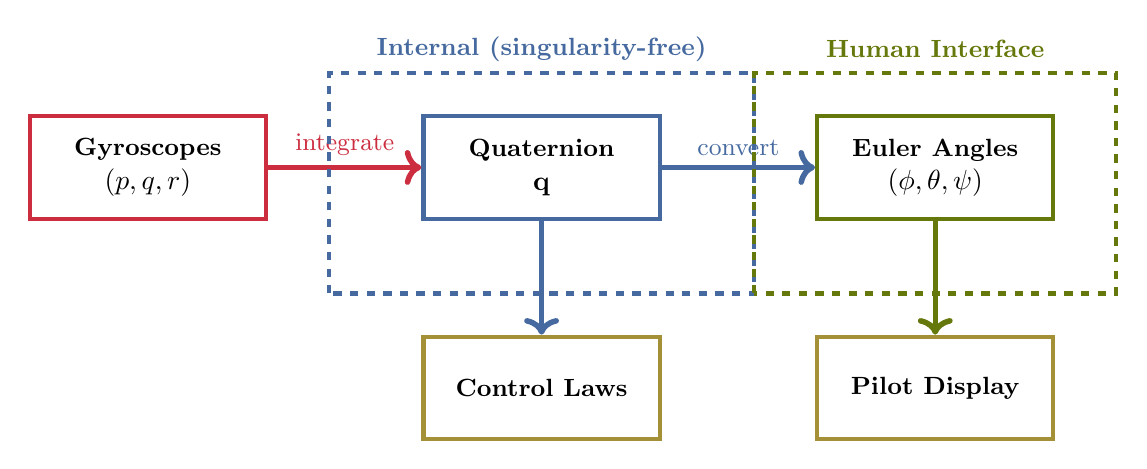
\begin{tikzpicture}[scale=1.0,
    block/.style={draw, line width=1.5pt, fill=white, minimum width=3cm, minimum height=1.3cm, sharp corners, align=center}]

    % Blocks
    \node[block, draw=USC_Rose] (gyro) at (0,0) {\small \textbf{Gyroscopes}\\$(p,q,r)$};
    \node[block, draw=USC_Blue] (quat) at (5,0) {\small \textbf{Quaternion}\\$\mathbf{q}$};
    \node[block, draw=USC_Olive] (euler) at (10,0) {\small \textbf{Euler Angles}\\$(\phi,\theta,\psi)$};
    \node[block, draw=USC_Gold] (display) at (10,-2.8) {\small \textbf{Pilot Display}};
    \node[block, draw=USC_Gold] (control) at (5,-2.8) {\small \textbf{Control Laws}};

    % Arrows
    \draw[->, line width=2pt, USC_Rose] (gyro) -- (quat) node[midway, above, font=\small] {integrate};
    \draw[->, line width=2pt, USC_Blue] (quat) -- (euler) node[midway, above, font=\small] {convert};
    \draw[->, line width=2pt, USC_Olive] (euler) -- (display);
    \draw[->, line width=2pt, USC_Blue] (quat) -- (control);

    % Annotations - dashed boxes
    \draw[dashed, USC_Blue, line width=1.5pt] (2.3,-1.6) rectangle (7.7,1.2);
    \node[USC_Blue, font=\small\bfseries] at (5,1.5) {Internal (singularity-free)};

    \draw[dashed, USC_Olive, line width=1.5pt] (7.7,-1.6) rectangle (12.3,1.2);
    \node[USC_Olive, font=\small\bfseries] at (10,1.5) {Human Interface};
\end{tikzpicture}
\end{document}
